\documentclass{beamer}
\usepackage{cmap}
\usepackage[utf8]{inputenc}
\usepackage[russian]{babel}
\usepackage{listings}
\usetheme{Antibes}
\usecolortheme{beaver}
\usepackage{graphicx}
\graphicspath{{img/}}

\title{Вероятностная модель токенизации в проекте Открытый корпус}
\author{В.\,В.~Бочаров\andД.\,В.~Грановский\andА.\,В.~Суриков\\\small\it Mathlingvo}
\date{18~апреля 2012~г.}
\begin{document}

% title page
\maketitle

%slide 01
\begin{frame}
\frametitle{Жизненный цикл текста}
\begin{enumerate}
\item{Исходный текст}
    \begin{itemize}
    \item{под лицензией, совместимой с CC-BY-SA}
    \item{проходит вычитку}
    \item{делится на абзацы, предложения и токены}
    \end{itemize}
\pause
\item{Морфологические интерпретации}
    \begin{itemize}
    \item{словарь на базе словаря проекта АОТ}
    \item{но морфологический стандарт~--- свой}
    \item{генерируются все возможные гипотезы}
    \end{itemize}
\pause
\item{Ручное снятие неоднозначности пользователями}
\pause
\item{Разметка доступна для просмотра и скачивания}
\end{enumerate}
\end{frame}

%slide 02
\begin{frame}
\frametitle{Уровни текста}
Концептуальные уровни:
\begin{enumerate}
\item{Графематика}
\item{Морфология}
\item{Синтаксис} (в отдаленных планах)
\item{Семантика} (в совсем отдаленных планах)
\item{Something else?}
\end{enumerate}
\pause
4 иерархических уровня деления (это графематика):
\begin{enumerate}
\item{Текст}
\item{Абзац}
\item{Предложение}
\item{Токен*}
\end{enumerate}
* некоторая последовательность символов без пробелов
\end{frame}

%slide 03
\begin{frame}
\frametitle{Токенизация}
Как разделить текст на эти единицы?
\begin{itemize}
\item{на абзацы~-- взять из источника}
\pause
\item{на предложения~-- пока вручную}
\pause
\item{на токены~-- полуавтоматически}
\end{itemize}
\end{frame}

%slide 03.1
\begin{frame}
\frametitle{Токенизация}
Токенизация должна быть:
\begin{itemize}
\item{единообразной}
\item{удобной для морфологии}
\end{itemize}
Проблемы ручной токенизации:
\begin{itemize}
\item{очень трудоемко}
\item{трудно обеспечить единообразие}
\item{не все отличия видны глазами}
\end{itemize}
\end{frame}

%slide 04
\begin{frame}
\frametitle{Токенизация-2}
Используем простое машинное обучение:
\begin{itemize}
\item{корпус предложений, уже разделенных на токены (внутри текста расставлены границы)}
\pause
\item{набор бинарных характеристических функций (15 шт.)} \\
F1 = <<является ли данный символ пробелом>> \\
... \\
F7 = <<является ли данный символ буквой кириллицы>> \\
... \\
F15 = <<является ли цепочка символов от ближайшего пробела слева до ближайшего пробела справа словарным словом>>
\pause
\item{вычисляем все эти функции для каждой позиции в предложении}
\end{itemize}
\end{frame}

%slide 05
\begin{frame}
\frametitle{Токенизация-3}
Используем простое машинное обучение:
\begin{itemize}
\item{для каждой позиции получается двоичный вектор} \\
Позиция 1: 001000010000000 \\
Позиция 2: 100000100000010 \\
...
\pause
\item{для каждой позиции знаем, проходит ли в ней граница токенов}
\pause
\item{для каждого двоичного вектора на корпусе вычисляется вероятность того, что в позиции с таким вектором есть граница токенов}
\pause
\item{в реальном тексте в каждой позиции тоже вычисляем вектор и смотрим вероятность}
\end{itemize}
\end{frame}

%slide 06
\begin{frame}
\frametitle{Токенизация-4}
Так выглядит обучение:
\begin{figure}
\center{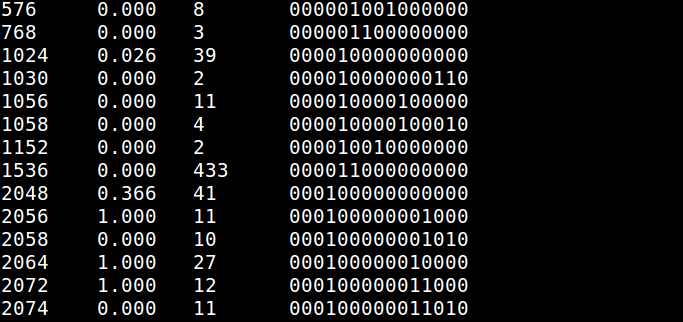
\includegraphics[width=1\linewidth]{2011_nlpseminar_1.png}}
\end{figure}
\end{frame}

%slide 07
\begin{frame}
\frametitle{Токенизация-5}
Получаемое деление~-- вероятностное, поэтому его нужно проверять глазами:
\begin{figure}
\center{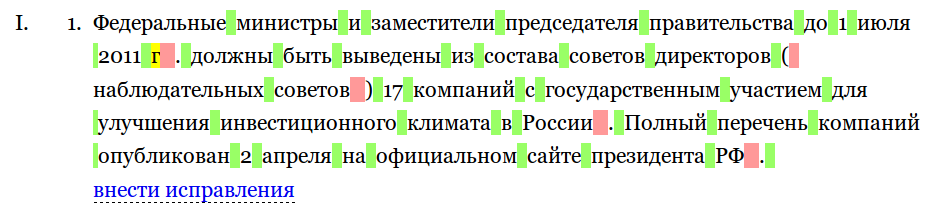
\includegraphics[width=1\linewidth]{2011_nlpseminar_2.png}}
\end{figure}
\pause
\begin{figure}
\center{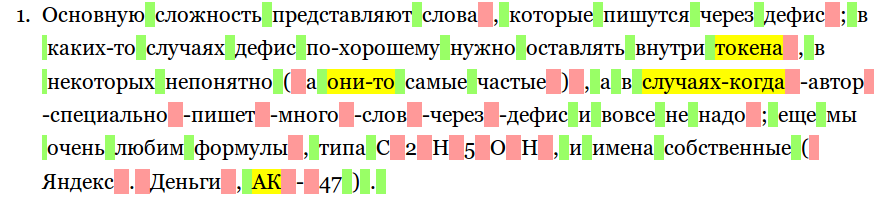
\includegraphics[width=1\linewidth]{2011_nlpseminar_3.png}}
\end{figure}
\end{frame}

%slide 08
\begin{frame}
\frametitle{Оценка качества}
\begin{itemize}
\item{Полнота / точность / F1 мера в зависимости от порога}
\begin{figure}
\center{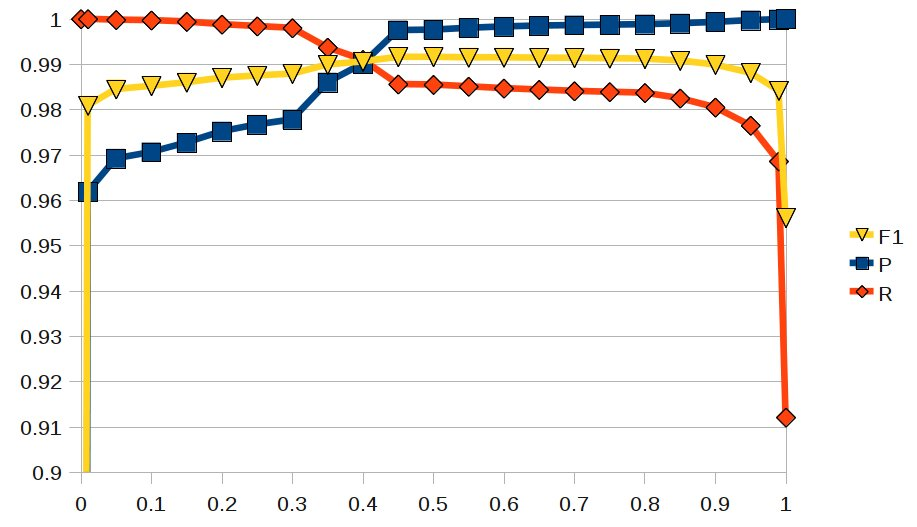
\includegraphics[width=1\linewidth]{2012_miem_3.png}}
\end{figure}
\end{itemize}
\end{frame}

%slide 09
\begin{frame}
\frametitle{Оценка качества}
\begin{itemize}
\item{При оценке не учитываются "очевидные" границы по пробелу}
\pause
\item{F1 = 99.15\% при значении порога 0.45 - 0.5}
\pause
\item{Для сравнения} \\
Правила \\
1. всегда разбивать по пробелам \\
2. всегда разбивать по границе буква / не буква \\
Дают F1 = 92\%
\end{itemize}
\end{frame}

%slide 09
\begin{frame}
\frametitle{Модуль на Perl}
\begin{itemize}
\item{Повторяет поведение токенизатора на OpenCorpora.org}
\pause
\item{Выложен на CPAN Lingua::RU::OpenCorpora::Tokenizer}
\pause
\item{Модель токенизации может обновляться}
\pause
\item{Прост в использовании:}
\begin{figure}
\center{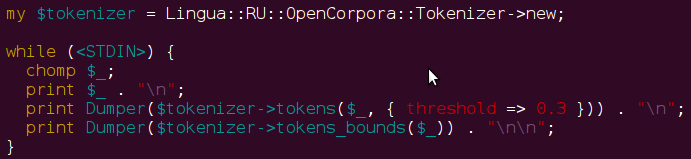
\includegraphics[width=1\linewidth]{2012_miem_1.png}}
\end{figure}
\end{itemize}
\end{frame}

%slide 10
\begin{frame}
\frametitle{Модуль на Perl}
\begin{itemize}
\item{Результат работы модуля:}
\begin{figure}
\center{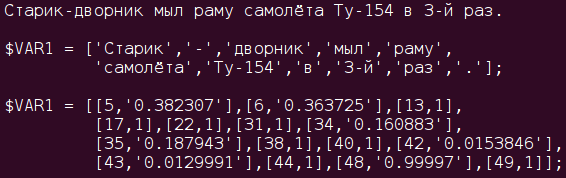
\includegraphics[width=1\linewidth]{2012_miem_2.png}}
\end{figure}
\end{itemize}
\end{frame}

%slide 10
\begin{frame}
\frametitle{Планы}
\begin{itemize}
\item{Графематика: Определение границ предложений, идентификация цитат и прямой речи}
\pause
\item{Морфология: Снятие морфологической омонимии}
\end{itemize}
\end{frame}

%slide 10
\begin{frame}
\frametitle{Морфологический разбор предложения по словарю}
\begin{figure}
\center{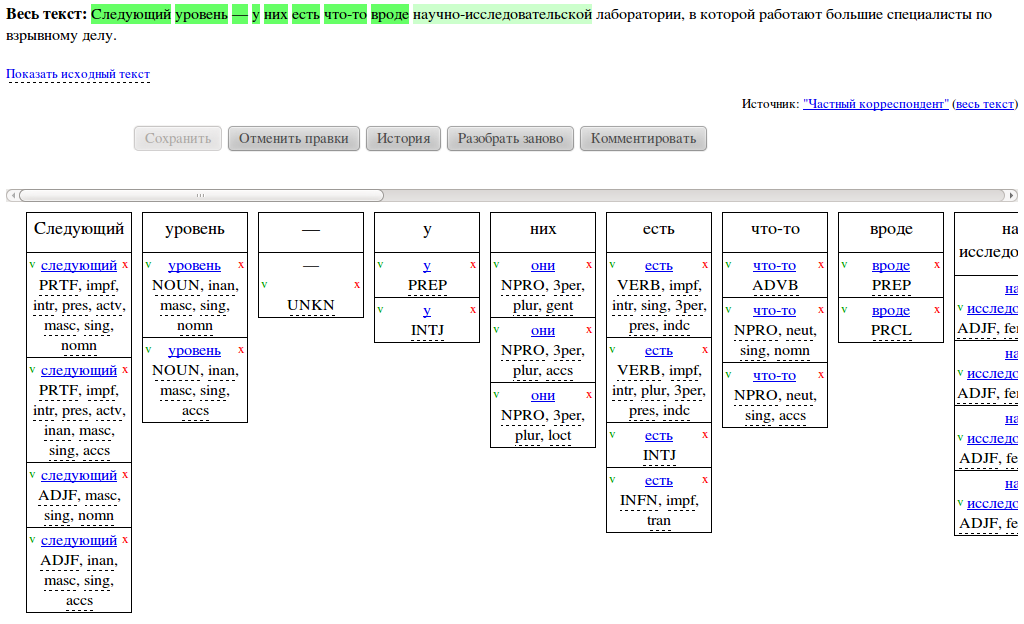
\includegraphics[width=1\linewidth]{2012_miem_5.png}}
\end{figure}
\end{frame}

%slide 10
\begin{frame}
\frametitle{Задание по снятию омонимии}
\begin{figure}
\center{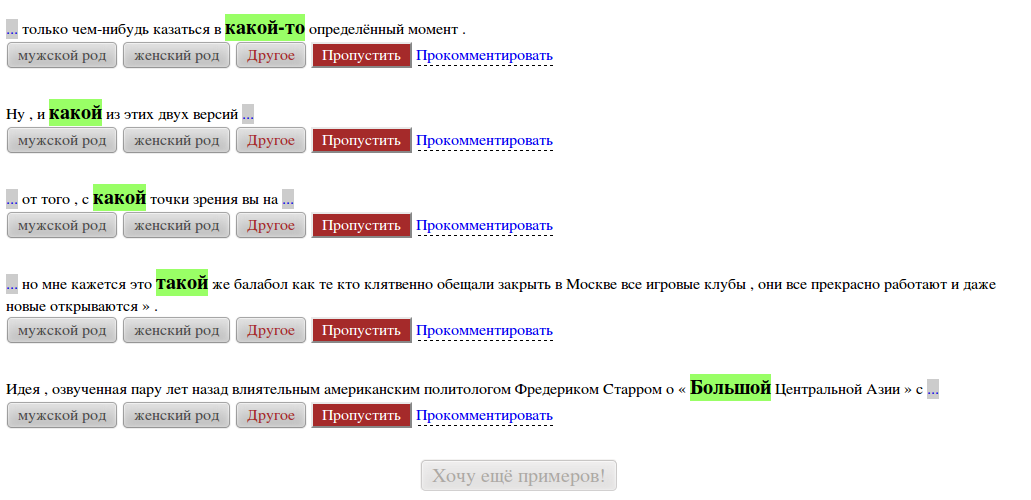
\includegraphics[width=1\linewidth]{2012_miem_4.png}}
\end{figure}
\end{frame}

%slide 10
\begin{frame}
\frametitle{Модерация результатов выполнения заданий}
\begin{figure}
\center{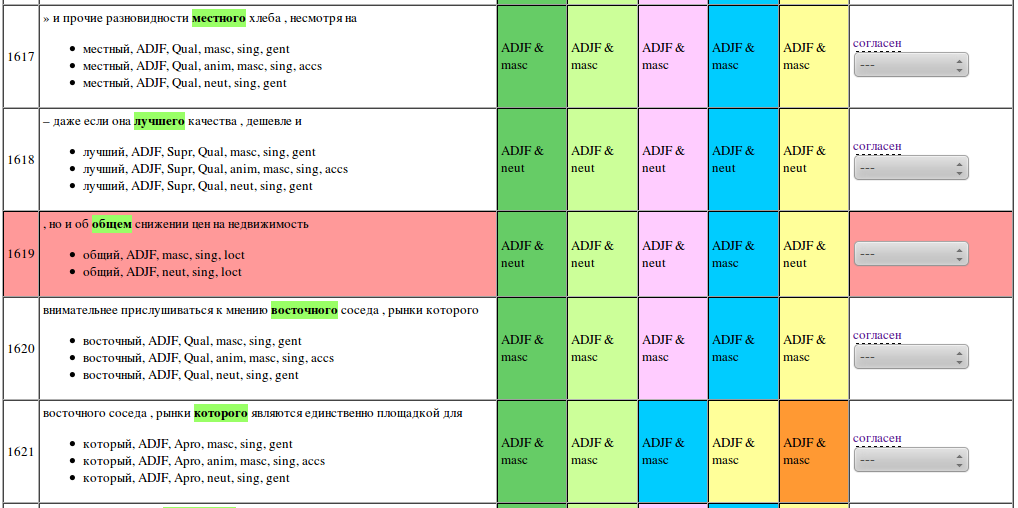
\includegraphics[width=1\linewidth]{2012_miem_6.png}}
\end{figure}
\end{frame}

%slide 08
\begin{frame}
Вопросы?
\end{frame}

%slide 09 
\begin{frame}
\frametitle{Contacts}
\begin{center}
\LARGE http://opencorpora.org\\[\bigskipamount]
\Large\texttt{granovsky@opencorpora.org\\bocharov@opencorpora.org}
\end{center}
\end{frame}

\end{document}
